% 報告会テンプレート(LuaLaTeX対応版)
\documentclass[10pt,a4j,twocolumn]{ltjsarticle}


\usepackage{graphicx}   % \includegraphics を使うためのパッケージ読み込み
\usepackage{imcreport}  % IMC報告会用テンプレートパッケージの読み込み

\usepackage{newtxmath}
\usepackage{amsmath,amssymb}
\usepackage{bm}

% ハイフネーションを抑制する.数値が大きいほど,無理にでも抑制しようとする.
\hyphenpenalty=10000\relax
\exhyphenpenalty=10000\relax
\sloppy


\title{不確かさを持つマニピュレータの動的可操作性の性質調査} % タイトル
\author{高谷秀明}                              % 著者
\studentnumber{TD18K001}                         % 学籍番号
\date{2019--05--24}                              % 日付
\header{中間報告}                                % 左上のヘッダ内容


\begin{document}

\maketitle

\section{はじめに}

前回の報告書では不確かさを持つ静的マニピュレータの可操作性の振る舞いを調べ,不確かさが可操作性へ及ぼす影響はほとんどないと結論づけた.
今回は不確かさを持つ動的マニピュレータを導入し,不確かさが動的可操作性に与える影響を調査した.

\section{動的マニピュレータと動的可操作性}

手先座標$\bm{r} \in \mathbb{R}^{n}$についての運動学モデルおよびリンク角度$\bm{q} \in \mathbb{R}^{m}$についての動力学モデルが次式で与えられるマニピュレータを考える.
\begin{equation}
  \bm{r} = \bm{f}(\bm{q}),
  \quad
  \bm{M}(\bm{q}) \ddot{\bm{q}} + \bm{H}(\bm{q}, \dot{\bm{q}}) + \bm{G}(\bm{q}) = \bm{\tau},
  \label{eq:models}
\end{equation}
ここで$\bm{M}$は慣性行列であり,マニピュレータの動特性の大きさを表す.

式~\eqref{eq:models}のマニピュレータについての動的可操作性$w_{d}$は次式で定義される.
\begin{equation}
  w_{d}(\bm{\theta}) \triangleq \left. \sqrt{\det\left(\bm{J}\left(\bm{M}^{\mathrm{T}}\bm{M}\right)^{-1}\bm{J}^{\mathrm{T}}\right)} \right|_{\bm{q}=\bm{\theta}},
  \label{fig:dynamic_manipulability}
\end{equation}
ここで$\bm{J}(\bm{q}) = [\partial r_{i} / \partial q_{j}]_{1 \leq i \leq n, 1 \leq j \leq m}$はマニピュレータのヤコビアンである.
$w_{d}$は$\|\bm{\tau}\| \leq 1$を満たす任意のトルクで実現可能な全ての手先加速度$\ddot{\bm{r}}$で構成される多面体の体積を表す.
$w_{d}(\bm{\theta})$の値が大きいことは姿勢$\bm{\theta}$におけるマニピュレータの運動性能が高いことを意味する.

\section{不確かさを取り入れた動的可操作性}

式~\eqref{eq:models}のマニピュレータが不確かさを持つ,すなわち不確かさを表す確率変数$\bm{\xi}$を含むとき,動的可操作性は姿勢と不確かさの関数へ拡張される.
\begin{equation}
  \bm{J}(\bm{q}) \mapsto \bm{J}(\bm{q}, \bm{\xi}), \quad
  \bm{M}(\bm{q}) \mapsto \bm{M}(\bm{q}, \bm{\xi}) \Rightarrow
  w_d(\bm{\theta}) \mapsto w_d(\bm{\theta}, \bm{\xi}).
  \label{eq:expansion}
\end{equation}
このとき動的可操作性の期待値および標準偏差が定義される.
期待値は式~\eqref{fig:dynamic_manipulability}と同様に運動性能の高さを表し,
標準偏差は不確かさが$w_{d}$の値に及ぼす影響の大きさを表すと解釈できる.

\section{拡張動的可操作性の検証}

式~\eqref{eq:expansion}の拡張された動的可操作性の挙動を調べるために,物体を把持した平面3リンクマニピュレータを考える.
把持物の質量には不確かさが存在するものとする.
このとき各リンク角度が$q_{1} = -q_{2}, 0 \leq q_{2} \leq 180, 0 \leq q_{3} \leq 180$ [deg]であるときの拡張動的可操作性の期待値と標準偏差を図~\ref{fig:dyman_mean_std_2d}に示す.
\begin{figure}
  \centering
  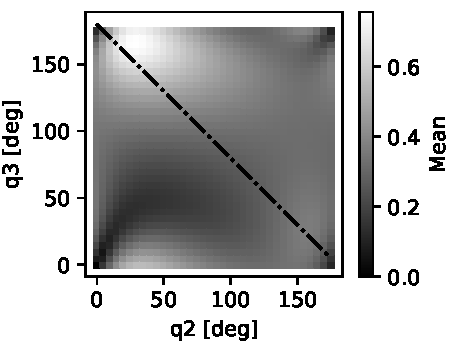
\includegraphics[width=60truemm]{./dm_mean.pdf}
  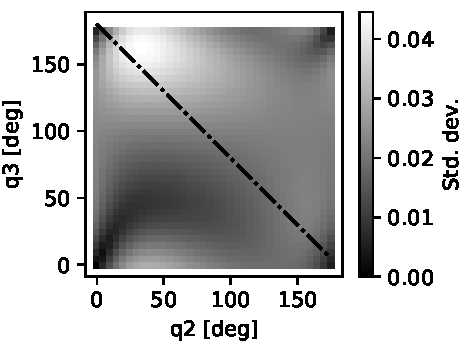
\includegraphics[width=60truemm]{./dm_std.pdf}
  \caption{動的可操作性の期待値(上)と標準偏差(下)}
  \label{fig:dyman_mean_std_2d}
  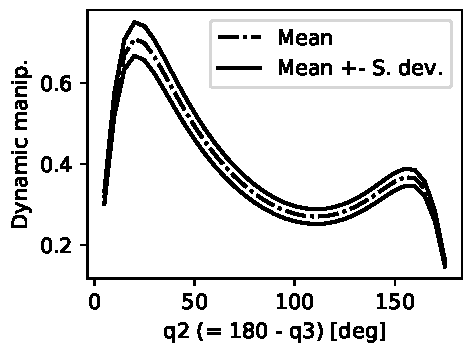
\includegraphics[width=60truemm]{./dm_dist.pdf}
  \caption{図~\ref{fig:dyman_mean_std_2d}の一点鎖線に沿ってプロットした動的可操作性}
  \label{fig:dyman_mean_std_1d}
\end{figure}
図から期待値と標準偏差がほとんど同様の傾向を示していることが確認できる.

図中の一点鎖線は同じ手先位置$(x, y) = (1, 0)$ [m]を指す姿勢を示している.
この線に沿ってプロットした期待値と標準偏差を図~\ref{fig:dyman_mean_std_1d}に示す.
期待値の変化量に比べて標準偏差の変化量は小さいため,不確かさが動的可操作性に及ぼす影響は姿勢の影響に比べて無視できる.
前報告会の結果と今回の結果より,不確かさの影響を表す指標として可操作性を用いるのは合理的でないと結論づける.

\end{document}
